\section{L'ordonnancement cumulatif}
\label{sec:cumu}

\subsection{L'ordonnancement en programmation par contraintes}
\label{sec:cumu_ordo}

Les problèmes d'ordonnancement étudiés en programmation par
contraintes sont majoritairement regroupés en trois catégories: les
problèmes préemptifs, les problèmes non préemptifs et les problèmes
élastiques. Les problèmes préemptifs (respectivement non préemptifs)
sont des problèmes pour lesquels l'interruption des activités est
autorisée (resp. non autorisée). Les {\it problèmes d'ordonnancement
élastiques} correspondent aux problèmes où la quantité de ressource
attribuée à une activité peut varier, à tout instant $t$ de l'horizon
de temps, avec la contrainte que la quantité totale de ressource
consommée par l'activité durant son exécution soit égale à une
certaine valeur appelée {\it énergie}. Cette dernière notion peut
aisément être étendue dans le cas où l'énergie reçue par une activité
n'est pas égale à la quantité de ressource consommée mais où des
fonctions de rendement modélisent cette conversion. Clairement, le
\CECSP~est un exemple typique d'un tel problème. Dans la suite de ce
chapitre, nous considérons la notion d'énergie au sens de la quantité
totale de ressource consommée. L'extension de cette notion pour
prendre en considération les fonctions de rendement sera détaillée
dans le chapitre~\ref{sec:PPC_CECSP}.

La majorité des problèmes d'ordonnancement non préemptifs classiques
peuvent être modélisés à l'aide d'un problème de satisfaction de
contraintes. En général, trois variables représentant respectivement
la date de début d'une activité, notée $st_i$, sa date de fin, notée
$et_i$ et sa durée, notée $p_i$, sont définies. Les domaines de
chacune de ces variables sont définis par les données du problème. En
effet, pour chaque activité, nous pouvons calculer une date de début
au plus tôt, $\ES$, et au plus tard, $\LS$; ainsi, le domaine de la
variable $st_i$ est $[\ES,\LS]$. De même, le domaine de la variable
$et_i$ est $[\EE,\LE]$, avec $\EE$ la date de fin au plus tôt de $i$
et $\LE$ sa date de fin au plus tard. La durée d'une activité est
quant à elle définie comme la différence entre sa date de fin et sa
date de début, i.e. $p_i=et_i-st_i$.

Les problèmes préemptifs sont plus difficiles à modéliser. En effet,
dans ce cas-là, un ordonnancement valide peut être uniquement 
représenté par une date de début, de fin et une durée pour chaque
activité. Pour ces problèmes, au moins deux modélisations différentes
existent. La première consiste à associer à chaque activité une
variable d'ensemble, i.e. une variable dont la valeur sera un
ensemble. Cette variable représente l'ensemble des instants $t$ où
l'activité est en cours, défini comme un ensemble d'intervalles ou de
temps $t$ discret. Une seconde possibilité est de définir une variable
binaire, pour chaque activité et chaque instant $t$, qui prendra la
valeur $1$ si l'activité est en cours à l'instant $t$. Notons que,
dans le cas d'un problème d'ordonnancement continu, une telle solution
ne peut être envisageable car cela conduirait à un nombre infini de
telles variables.

Les problèmes élastiques sont, quant à eux, modélisés à travers les
contraintes de ressources. Il existe deux principaux types de
contraintes de ressource en PPC. Le premier permet de modéliser les
ressources disjonctives, i.e. qui ne peuvent exécuter qu'une seule
activité à un instant donné, et le second sert à la modélisation des
ressources cumulatives. Dans ce manuscrit, nous nous intéressons
seulement au second cas.

{\'E}tant donné une activité et une ressource de capacité $R$, une
variable $b_i$ sert généralement à modéliser la consommation de
l'activité sur cette ressource. Dans le cas des tâches élastiques,
cette variable est remplacée par une variable $W_i$ représentant
l'énergie requise par l'activité. Pour représenter un ordonnancement,
un ensemble de variables représentant la quantité de ressource
utilisée par une activité à l'instant $t$ est introduit. Ces variables
sont ensuite liées entre elles par un ensemble de contraintes
modélisant le fait que chaque activité doit recevoir une énergie
$W_i$. 

Ces différents concepts peuvent être étendus pour modéliser d'autre
types de contraintes telles que des contraintes de ressources
alternatives, des temps de préparation entre les activités, des
activités optionnelles ou des contraintes de réservoirs.

Dans la suite de ce manuscrit, nous nous intéressons aux problèmes
d'ordonnancement non préemptifs avec ressource cumulative et aux
problèmes d'ordonnancement élastiques. Le premier cas correspond au
\CUSP, décrit dans le paragraphe~\ref{sec:ordo_res}. En PPC, le
problème est modélisé à l'aide d'une contrainte globale appelée
contrainte cumulative. Cette contrainte ainsi que différents
algorithmes de filtrage mis en place pour cette dernière sont
présentés dans les deux paragraphes suivants. 

Les problèmes d'ordonnancement élastiques seront représentés par le
\CECSP~(voir paragraphe~\ref{sec:ordo_nrj}), pour lequel l'adaptation
de certains algorithmes de filtrage pour la contrainte cumulative est
présentée dans le chapitre~\ref{sec:PPC_CECSP}.

\subsection{La contrainte cumulative}
\label{sec:cumu_cume}

En PPC, le \CUSP~est modélisé par la contrainte cumulative. Dans ce
contexte, une activité est souvent représentée par $4$ variables:
$st_i,\ et_i,\ p_i$ et $b_i$ correspondant respectivement à la date de
début de l'activité, sa date de fin, sa durée et sa consommation de
ressource. En règle générale, les domaines des variables $p_i$ et
$b_i$ sont restreints à un seul élément, i.e. la durée de l'activité
est fixe et sa consommation de ressource est constante durant toute
son exécution. Les domaines des variables $st_i$ et $et_i$ sont quant
à eux considérés finis.

La contrainte cumulative vise donc à déterminer seulement les dates de
début et de fin des activités -- liés par la condition d'intégrité
$et_i=st_i+p_i$. Cette contrainte prend donc en paramètres l'ensemble
d'activités $\A$ à ordonnancer et la capacité $R$ de la ressource utilisée
pour exécuter les activités. Avec ces notations la contrainte s'écrit
$cumulative(\A,R)$ et cette contrainte est satisfaite si et seulement 
si:
\begin{align}
  \forall i \in \A, & \quad  st_i+p_i=et_i \label{eq:CUSP_int}\\
  \forall t \in \H, &\quad \sum_{\substack{i \in A\\t \in
  [st_i,et_i[}} b_i \le R  \tag{\ref{eq:CUSP_res}} 
\end{align}
La seconde contrainte ainsi qu'un exemple de solution sont détaillés
dans le paragraphe~\ref{sec:ordo_res}.

L'existence d'une solution au problème cumulatif étant un problème
NP-complet, un algorithme effectuant un filtrage complet des domaines
des variables, i.e. retirant toutes les valeurs incohérentes des
domaines des variables, ne peut s'exécuter en temps polynomial. De
plus, assurer seulement la cohérence des bornes des domaines étant
aussi NP-complet, les algorithmes utilisés permettent seulement
d'ajuster seulement certaines bornes des domaines en fonction des
données et contraintes du problème sans s'assurer de la cohérence de
toutes les bornes. Ces algorithmes de filtrage se présentent le plus
souvent sous la forme de règles, appelées {\it règles d'ajustement},
et sont appliqués sur des relaxations de la contraintes cumulative et
des règles pouvant être appliquées en temps polynomial ont été mises
en place pour des relaxations.

Dans ce manuscrit, nous présentons quelques une de ces
techniques. Pour une description plus détaillée des différentes
techniques de relaxation existantes pour la contrainte cumulative,
nous renvoyons le lecteur à~\cite{BLPN,DHP}. 
Baptiste {\it et al.}~\cite{BLPN} présentent un panorama de ces
différentes relaxations ainsi que les principales techniques issues de
la programmation par contraintes mises en place pour résoudre la
contrainte cumulative. Dans un contexte plus général, Dorndoff {\it et
al.}~\cite{DHP} exhibent des règles de cohérence basées sur la
capacité des intervalles, i.e. la quantité de ressource disponible
dans un intervalle.

Le paragraphe suivant présente plusieurs de ces règles d'ajustement
définies pour la contrainte cumulative. 


\subsection{Les filtrages de la contrainte cumulative}
\label{sec:cumu_propag}

Le problème cumulatif étant un problème symétrique, les règles
d'ajustement sont souvent définies pour une seule des deux variables
$st_i$ et $et_i$. En effet, une fois ces règles étant définies pour
une de ces deux variables, les règles symétriques peuvent être
déduites pour l'autre variable. Les raisonnements et algorithmes
décrits dans ce paragraphe ne présentent que le filtrage du début au
plus tôt.

Dans un premier temps, nous présentons des règles simples permettant
l'ajustement des bornes des variables. Ensuite, une partie sera
consacrée aux règles d'ajustement basées sur le concept
d'énergie. Enfin, ces règles seront combinées afin de créer
des algorithmes permettant un filtrage plus fort des domaines des
variables.

Plusieurs des règles présentées dans ce paragraphe seront ensuite
adaptées dans le cas du \CECSP~dans le chapitre~\ref{sec:PPC_CECSP}.

\subsubsection{Règles de filtrages simples}

Parmi les raisonnements les plus simples appliqués dans le cadre de la
contrainte cumulative, on retrouve le raisonnement basé sur
l'échéancier (on utilise le terme anglais de Time-Table)~\cite{TTLah}
et le raisonnement disjonctif~\cite{BLPN}.

\paragraph{Time-Table}
Le premier algorithme de filtrage de la contrainte cumulative
présenté est basé sur la notion de {\it partie obligatoire} d'une
activité. Cette partie obligatoire correspond à l'intervalle de temps
maximal pendant lequel on est sûr que l'activité devra être
exécutée. Cet intervalle est vide dans le cas où $\LS \ge \EE$, et est
égal à $[\LS,\EE{[}$ dans le cas contraire. Notons que dans le cas de la
contrainte cumulative, une borne supérieure sur la date de début d'une
activité peut aisément être calculée. En effet, il suffit de prendre
$\LS=\LE - p_i$. 


\begin{defi}
La partie obligatoire d'une activité $i$ est définie par l'intervalle
$[\LS,\EE{[}$.
\end{defi}

\begin{ex}
Considérons l'activité suivante: 

\vspace{-0.5cm}
\begin{center}
  \begin{tabular}{|P{1cm}P{1cm}P{1cm}P{1cm}|}
    \hline
    \ES & \LE & p_i & b_i  \\
    \hline
    1 & 13 & 8 & 2 \\
    \hline
  \end{tabular}
\end{center}

Nous pouvons calculer sa date de début au plus tard,
$\LS=\LE - p_i=13-8=5$, ainsi que sa date de fin au
plus tôt, $\EE=\ES + p_i=1+8=9$. Comme $\EE > \LS$,
l'activité possède une partie obligatoire qui est l'intervalle $[5,9[$
(voir figure~\ref{fig_mand_CUSP}).
  
\begin{figure}[htb!]
\subcaptionbox{Ordonnancement au plus tôt}[0.3\linewidth]{
    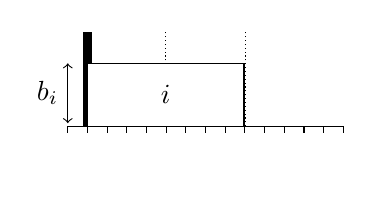
\begin{tikzpicture}
      [xscale=0.25, yscale= 0.4,node distance=0.5cm]
      \node (sil) at (1,0) {} ;
      \node (eil) at (9,0) {} ;
      \node [below of=eil,node distance=0.63cm]  {$\EE$};
      \draw (sil.center) node[below=0.2cm] {$\ES$};
   \node (sir) at (5,0) {} ;
      \node (eir) at (13,0) {} ;
      \node[below of= sir,node distance=0.63cm] {$\LS$};
      \draw (eir.center) node[below=0.2cm] {$\LE$};
      
      \draw (0,0) -- (14,0);
      \draw[line width=3pt] (1,0) -- (1,3);
      
      \draw[densely dotted] (9.05,0) -- (9.05,3);
     \draw[densely dotted] (4.95,0) -- (4.95,3);
      \draw[<->] (0,0.1) -- (0,2) node[midway,left] {$b_i$};
      \draw[fill=white] (1,0) rectangle (8.95,2) node[midway] {$i$};

      \foreach \i in {0,...,14} {
        \draw (\i,0)  -- (\i,-0.2);
      }
    \end{tikzpicture}
}
\hfill
\subcaptionbox{Ordonnancement au plus tard}[0.3\linewidth]{
    \begin{tikzpicture}
      [xscale=0.25, yscale= 0.4,node distance=0.5cm]
        \node (sil) at (1,0) {} ;
      \node (eil) at (9,0) {} ;
      \node [below of=eil,node distance=0.63cm]  {$\EE$};
      \draw (sil.center) node[below=0.2cm] {$\ES$};
   \node (sir) at (5,0) {} ;
      \node (eir) at (13,0) {} ;
      \node[below of= sir,node distance=0.63cm] {$\LS$};
      \draw (eir.center) node[below=0.2cm] {$\LE$};
      
      \draw (0,0) -- (14,0);
      \draw[line width=3pt] (13,0) -- (13,3);
      
      \draw[densely dotted] (4.95,0) -- (4.95,3);
      \draw[densely dotted] (9.05,0) -- (9.05,3);
      \draw[<->] (14,0.1) -- (14,2) node[midway,right] {$b_i$};
      \draw[fill=white] (5.05,0) rectangle (13,2) node[midway] {$i$};

      \foreach \i in {0,...,14} {
        \draw (\i,0)  -- (\i,-0.2);
      }
    \end{tikzpicture}
}
\hfill
\subcaptionbox{Partie obligatoire}[0.3\linewidth]{ 
  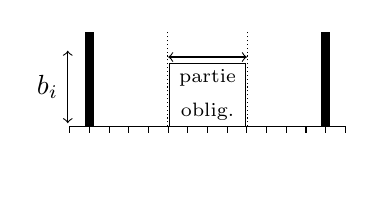
\begin{tikzpicture}
    [xscale=0.25, yscale= 0.4,node distance=0.5cm]
    \node (sir) at (5,0) {} ;
    \node (eil) at (9,0) {} ;
    \node [below of=eil,node distance=0.63cm]  {$\EE$};
    \node[below of= sir,node distance=0.63cm] {$\LS$};
    \draw[<->] (5,2.2) -- (9,2.2) node[midway,label={}]
    {};
    
    \draw (5.05,0) rectangle (8.95,2)
    node[midway,color=black,align=center,text width=1.4cm]
    {\scriptsize partie oblig.}; 
    
    
    \draw (0,0) -- (14,0);
    \draw[line width=3pt] (1,0) -- (1,3);
    \draw[line width=3pt] (13,0) -- (13,3);
    
    \draw[<->] (-0.1,0.1) -- (-0.1,2.4) node[midway,left] {$b_i$};

    \draw[densely dotted] (4.95,0) -- (4.95,3);
    \draw[densely dotted] (9.05 ,0) -- (9.05,3);

    \foreach \i in {0,...,14} {
      \draw (\i,0)  -- (\i,-0.2);
    }
  \end{tikzpicture}
}
\caption{Partie obligatoire d'une activité $i$ pour le \CUSP.}
\label{fig_mand_CUSP}
\end{figure}
\end{ex}

Les parties obligatoires des activités peuvent ensuite être agrégées de
manière à obtenir une fonction en escalier, appelée {\it profil
  obligatoire de la ressource}.  

\begin{defi}
\label{def:profil_oblig}
  Le {\bf profil obligatoire}  $TT_{\cal A}$ d'une ressource est défini
  par la fonction suivante: $TT_{\cal A}(t)= \sum_{\substack{i \in {\cal
        A}\\ \LS \le t < \EE}} b_i ,\ \forall t \in \H$.  Le problème n'admet
  pas de solution si $\exists t \in \H \ : \ TT_{\cal A}(t) > R$.
\end{defi}


\begin{ex}
  \begin{figure}[!htb]
    \centering
    \begin{tikzpicture}
      [yscale=0.45,xscale=0.6]
      \node (O) at (0,0) {};
      \foreach \i in {0,...,13} {
        \draw (\i-1,0) -- (\i-1,-0.1) node[below] {$\i$};
      }
      
      \draw (0,0) -- (0,2) -- (2,2) -- (2,4) -- (4,4) -- (4,6) --
      (5,6) -- (5,1) -- (9,1) -- (9,3) -- (11,3) -- (11,0);
      \draw[->] (-1,0) -- (12.5,0) node[below] {$t$};
      \draw[dashed] (-1,5) -- (12.5,5);
      \draw[->] (-1,0) -- (-1,5.5) node[left] {$R=5$};
    \end{tikzpicture}
    \caption{Exemple de profil obligatoire d'une ressource cumulative.}
    \label{fig_profil_CUSP}
  \end{figure}
  Dans l'exemple décrit par la figure~\ref{fig_profil_CUSP}, nous
  remarquons que, au temps $t=1$, le profil obligatoire de la
  ressource vaut $2$. Comme la ressource est de capacité $5$, aucune
  incohérence n'est détectée. À l'inverse, au temps $t=5$, le profil
  obligatoire de la ressource a une valeur de $6$, ce qui est
  supérieur à la capacité de la ressource. Une incohérence est donc
  détectée et il n'existe pas de solution réalisable pour cette
  instance. 
\end{ex}

Pour réaliser un filtrage des bornes, nous devons fournir des règles
permettant d'identifier si débuter l'activité $i$ à $\ES$ (ou $\LS$)
ne viole pas les contraintes du problème. Cette règle peut être
formalisée de la façon suivante: 

\begin{reg}
\label{reg:TT}
Soit une activité $i \in \A$. S'il existe $t \in [\ES,\LS{[}$ tel que
$t < \EE$ et que $b_i + TT_{\A \setminus\{i\}}(t) > R$ alors la date
de début au plus tôt de $i$ peut être ajustée et on a: $ \ES > t$.
\end{reg}

\begin{ex}
 Soit l'activité définie ci-dessous.
\begin{center}
  \begin{tabular}{|P{1cm}P{1cm}P{1cm}P{1cm}|}
    \hline
    \ES & \LE & p_i & b_i  \\
    \hline
    1 & 14 & 8 & 2 \\
    \hline
  \end{tabular}
\end{center}
La figure~\ref{fig:TT_CUSP} présente le profil obligatoire de la
ressource ainsi que l'ajustement déduit de la règle~\ref{reg:TT}.
  \begin{figure}[!htb]
    \centering
    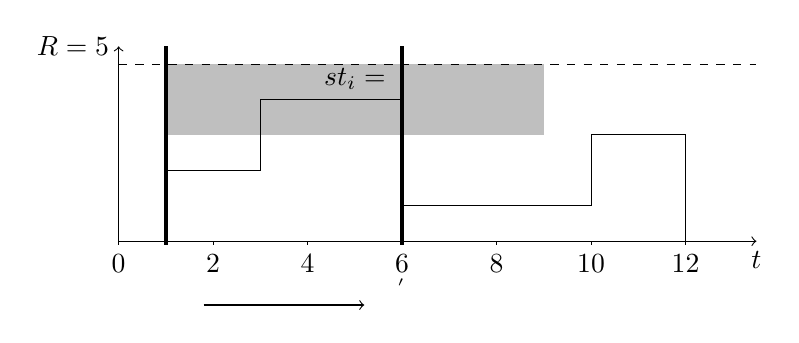
\begin{tikzpicture}
      [yscale=0.45,xscale=0.6]
      \node (O) at (0,0) {};
      \foreach \i in {0,2,...,13} {
        \draw (\i-1,0) -- (\i-1,-0.1) node[below] {$\i$};
      }
      
      \fill[draw=black,gray!50] (0,5) rectangle (8,3) node[midway,above,color=black]
      {$st_i=\ES$};
      \draw (0,0) -- (0,2) -- (2,2) -- (2,4) -- 
      (5,4) -- (5,1) -- (9,1) -- (9,3) -- (11,3) -- (11,0);
      \draw[->] (-1,0) -- (12.5,0)  node[below] {$t$};
      \draw[dashed] (-1,5) -- (12.5,5);
      \draw[->] (-1,0) -- (-1,5.5) node[left] {$R=5$};
      \draw[very thick=3pt] (0,-0.1) node[below=0.4cm] {$\ES$}-- (0,5.5);
      \draw[very thick=3pt] (5,-0.1) node[below=0.3cm] {$\ES^{'}$}-- (5,5.5);
      \draw[->] (0.8,-1.8) -- (4.2,-1.8);
    \end{tikzpicture}
    \caption{Règle d'ajustement du Time-Table pour le \CUSP.}
    \label{fig:TT_CUSP}
  \end{figure}
Dans cet exemple, on voit bien que l'activité ne peut pas commencer à
tout temps $t\in [\ES,6[$. En effet, le profil obligatoire de la ressource
montre que la quantité de ressource disponible dans l'intervalle
$[3,6[$ ne permet pas d'exécuter l'activité pendant cet intervalle. La
date de début au plus tôt peut donc être mise à jour ($\ES^{'}=6$).
\end{ex}

Beldiceanu {\it et al.}~\cite{BC} ont introduit un algorithme de
balayage permettant d'appliquer les ajustements décrits ci-dessus en
$O(n^2)$. D'autres algorithmes ont aussi été mis en place pour ce
raisonnement~\cite{OQ,LBC,GHS}. Ces algorithmes possèdent des
complexités théoriques moins élevées ou équivalentes avec l'algorithme
de balayage de Beldiceanu {\it et al.} en proposant des filtrages
moins importants.

\paragraph{Raisonnement disjonctif}
Une deuxième règle permettant d'ajuster les bornes des variables
repose sur un raisonnement appelé le {\it raisonnement disjonctif}. Ce
raisonnement est brièvement décrit dans~\cite{BLPN} et présenté plus
en détail dans~\cite{Gay2015}. 

Ce raisonnement repose sur le concept d'ensembles disjonctifs. Ces
ensembles correspondent aux ensembles d'activités qui ne peuvent
s'exécuter en parallèle. Son application la plus basique s'intéresse
seulement aux ensembles de taille $2$, c'est-à-dire aux paires
d'activités disjonctives. 

Si nous considérons deux activités $(i,j) \in \A^2$ telles que
$b_i+b_j > R$ alors une des deux affirmations suivantes doit être
vérifiée:
\begin{itemize}
\item l'activité $i$ doit commencer après la fin de l'activité $j$;
\item l'activité $i$ doit finir avant le début de l'activité $j$.
\end{itemize}
En effet, comme les activités $i$ et $j$ ne peuvent être exécutées en
parallèle, l'une doit forcément finir avant que l'autre ne puisse
s'exécuter.

Cette propriété nous permet d'améliorer les bornes des variables de
début d'activité selon la règle suivante:
\begin{reg}
  Soient $i,\ j \in \A$, $i\neq j$ telles que $b_i+b_j > R$ et $\LS
  <\EE[j]$. Alors la date de début au plus tôt de l'activité peut
  être ajustée et on a: $ \ES[j] \ge \EE$. 
\end{reg}

\begin{ex}
\label{ex:disj_CUSP}
Soient $i$ et $j$ les deux activités suivantes: 
\begin{center}
  \begin{tabular}{|P{1cm}|P{1cm}P{1cm}P{1cm}P{1cm}|}
    \hline
    act & \ES & \LE & p_i & b_i  \\
    \hline
   i & 2 & 11 & 4 & 2 \\
   j & 1 & 20 & 7 & 2 \\    
    \hline
  \end{tabular}
\end{center}

  \begin{figure}[htb!]
    \centering
    \begin{tikzpicture}
     \begin{scope} [yscale=0.45,xscale=0.4]
      \node (O) at (0,0) {};
      \foreach \i in {0,5,...,10} {
        \draw (\i,0) -- (\i,-0.1) node[below] {\small $\i$};
      }
      \fill[gray!50] (2,0) rectangle (11,2.4);
      \fill[gray!50] (1,2.6) rectangle (14,5);
      
      \draw[fill=white] (7,0.2) rectangle (11,2.2) node[midway]
      {$i$};
      \draw[fill=white] (1,2.8) rectangle (8,4.8) node[midway]
      {$j$};
      \draw[white, pattern=north west lines] (7,0) rectangle (8,5.5);

      \draw[->] (0,0) -- (14,0) node[below] {$t$};
      \draw[->] (0,0) -- (0,5.5) ;
      \draw (0,3) node[left] {$R=3$};
      \draw[densely dotted] (1,-0.1) -- (1,5.5) node[above] {$\ES[j]$};
      \draw[densely dotted] (8,-0.1) -- (8,5.5) node[above] {$\EE[j]$};
      \draw[densely dotted] (2,-0.1)  node[below] {$\ES$}-- (2,5.5);
      \draw[densely dotted] (6,-0.1 ) node[below=0.4cm] {$\EE$}-- (6,5.5) ;
      \draw[densely dotted] (7,-0.1) node[below] {$\LS$} -- (7,5.5) ;
      \draw[densely dotted] (11,-0.1) node[below right] {$\LE$} -- (11,5.5) ;
      % \draw[densely dotted] (6,-0.1) -- (6,5.5) node[above] {$\ES[j]^{'}$};
      % \draw[->] (1.8,5.8) -- (5.2,5.8);
    \end{scope}     
    \begin{scope} [yscale=0.45,xscale=0.4,xshift=20cm]
      \node (O) at (0,0) {};
      \foreach \i in {0,5,...,10} {
        \draw (\i,0) -- (\i,-0.1) node[below] {\small $\i$};
      }
      \fill[gray!50] (2,0) rectangle (11,2.4);
      \fill[gray!50] (6,2.6) rectangle (14,5);

      
      \draw[fill=white] (2,0.2) rectangle (6,2.2) node[midway]
      {$i$};
      \draw[fill=white] (6,2.8) rectangle (13,4.8) node[midway]
      {$j$};

      \draw[->] (0,0) -- (14,0) node[below] {$t$};
      \draw[->] (0,0) -- (0,5.5) ;
      \draw (0,3) node[left] {$R=3$};
      \draw[densely dotted] (6,-0.1) -- (6,5.5) node[above] {$\ES[j]$};
      \draw[densely dotted] (13,-0.1) -- (13,5.5) node[above] {$\EE[j]$};
      \draw[densely dotted] (2,-0.1)  node[below] {$\ES$}-- (2,5.5);
      \draw[densely dotted] (6,-0.1 ) node[below=0.4cm] {$\EE$}-- (6,5.5) ;
      \draw[densely dotted] (7,-0.1) node[below] {$\LS$} -- (7,5.5) ;
      \draw[densely dotted] (11,-0.1) node[below right] {$\LE$} -- (11,5.5) ;
      % \draw[densely dotted] (6,-0.1) -- (6,5.5) node[above] {$\ES[j]^{'}$};
      % \draw[->] (1.8,5.8) -- (5.2,5.8);
    \end{scope}
  \end{tikzpicture}
  \caption{Raisonnement disjonctif pour le \CUSP.}
  \label{fig:disj_CUSP}
\end{figure}
Dans l'exemple ci-dessus, nous avons $b_i+b_j=4 > 3$. Donc $i$ et $j$
ne peuvent s'exécuter en parallèle. Comme $\EE[j] = 8 > 7=\LS$, $i$
doit être exécutée avant $j$. En effet, $i$ doit forcément
démarrer avant $\LS=7$ et ,si $j$ est ordonnancée au plus tôt,
i.e. $st_j=\ES[j]=1$, $j$ ne peut finir avant $\EE[j]=8$. Donc, dans
ce cas, $i$ et $j$ se chevauchent. L'activité $j$ ne peut commencer à
$\ES[j]$ et doit commencer après $\EE=6$. Donc $\ES[j]$ est ajustée à
cette valeur.
\end{ex}

L'exemple~\ref{ex:disj_CUSP} montre que, dans certains cas, le
raisonnement disjonctif est plus fort que le Time-Table. En effet,
dans cet exemple, aucune des activités ne possède de partie
obligatoire. Aucun ajustement n'est donc détecté par la
règle~\ref{reg:TT}. 

{\`A} l'inverse, dans certains cas, le raisonnement Time-Table va
procéder à plus d'ajustements que le raisonnement disjonctif. En
effet, le raisonnement disjonctif présenté ici ne raisonne que sur des
paires d'activités tandis que le Time-Table est capable de détecter
des ajustements déduits de n-uplets d'activités. Il faut cependant que
les activités possèdent une partie obligatoire. Cependant, le
Time-Table est souvent plus utilisé en pratique car il peut amener les
mêmes déductions que les paires de disjonction tout en ayant une plus
faible complexité.

Dans le paragraphe~\ref{sec:mix_CUSP}, nous montrerons comme il est
possible de coupler ces deux raisonnements pour en obtenir un nouveau,
le Time-Table disjonctif~\cite{Gay2015}. 

Le paragraphe suivant est dédié aux règles de filtrage utilisant le
concept d'{\it énergie}. 
 
\subsubsection{Règles de filtrage énergétiques}
 \label{sec:nrj_CUSP}
Parmi les règles de filtrage utilisant le concept d'énergie on
retrouve le Edge-Finding\cite{VilimEF,theseNuijten}, le raisonnement
énergétique~\cite{RELopez} ou encore les activités
élastiques~\cite{BLPN}.  Nous présenterons en détail le second cas,
tandis que les autres cas seront brièvement discutés. La raison
principale étant que nous adapterons le raisonnement énergétique dans
le cas du \CECSP.

L'idée principale des raisonnements énergétique est de comparer la
quantité de ressource disponible dans un intervalle avec l'énergie que
doit consommer un ensemble de tâches à l'intérieur de ce même
intervalle. Les raisonnements diffèrent principalement sur la manière
de calculer cette énergie et sur les intervalles considérés. 

 Le raisonnement Edge-Finding s'applique sur un sous-ensemble
d'activités $\Omega \subseteq \A$, le but étant de décider si une
activité $j$ doit commencer avant $\Omega$ dans toute solution
réalisable. Dans ce cas, l'énergie d'une activité $i$ représente sa
charge de travail $W_i$ et est simplement exprimée comme
$W_i=p_i\times b_i$. L'énergie nécessaire pour un ensemble d'activités
$\Omega$ est alors $\sum_{i\in \Omega} W_i$. Les intervalles
considérés dans ce raisonnement correspondent aux fenêtres de temps des
activités $[\ES,\LE{[}$. Cette notion est étendue à $\Omega$ de la façon
suivante: $[\ES[\Omega],\LE[\Omega]{[}=[\min_{j \in \Omega}\ES[j],\max_{j
\in \Omega} \LE[j] {[}$. L'idée du raisonnement est alors  de vérifier
que la ressource disponible permet de faire débuter l'activité $i$
dans la fenêtre de temps correspondant à $\Omega$. Pour cela,
l'énergie requise par $\Omega \cup \{ i\}$ est comparée à la quantité
de ressource disponible dans l'intervalle $[\ES[\Omega],\LE[\Omega\cup
\{i\}]{[}$. Si la quantité de ressource n'est pas suffisante, alors
l'activité $i$ doit commencer avant $\ES[\Omega]$ et un ajustement
peut être effectué.

Dans le cas des activités partiellement et totalement élastiques, les
contraintes de consommation de ressource sont relâchées et une
activité n'est plus contrainte de consommer une quantité constante de
la ressource au cours du temps. Selon que l'activité est totalement
ou partiellement élastique, ces contraintes sont plus ou moins
relâchées et la consommation de ressource des activités peut subir des
variations plus ou moins grandes au cours du temps. L'avantage de ces
relaxations est que l'existence d'une solution peut être décidée en
temps polynomial. La façon dont les ajustements sont calculés étant
très similaire à celle dont ils sont calculés dans le cadre du
raisonnement énergétique, ils ne sont pas détaillés dans ce
manuscrit. Une description de ces ajustements peut être trouvé
dans~\cite{BLN}. 

Le raisonnement énergétique, introduit par~\cite{RELopez}, est un des
raisonnements les plus forts existant pour la contrainte
cumulative. Le principe est de considérer un intervalle $[t_1,t_2[$ et
de calculer l'énergie requise par une activité à l'intérieur de cet
intervalle. Dans ce cas, l'énergie requise par une activité dans un
intervalle $[t_1,t_2[$  équivaut à
la quantité minimale de ressource qu'elle doit utiliser
à l'intérieur de cet intervalle. Cette quantité, notée $\bb$, est
ensuite utilisée pour calculer la fonction de marge $SL(t_1,t_2)$
correspondant à la différence entre la quantité de ressource requise
par toutes les activités à l'intérieur de $[t_1,t_2[$ et la quantité
de ressource disponible dans ce même intervalle, $R (t_2-t_1)$. Si
cette quantité est négative pour un intervalle $[t_1,t_2[$, alors une
incohérence est détectée. En effet, si c'est le cas, alors cela
signifie que la quantité de ressource disponible dans $[t_1,t_2[$
n'est pas suffisante pour ordonnancer les consommations minimales de
toutes les activités.

\begin{defi}
La fonction de marge $SL(t_1,t_2)$ est définie de la façon suivante: 
\[  SL(t_1,t_2) = R (t_2-t_1) - \sum_{i \in \A} \bb \]
\end{defi}

Avec cette définition, nous pouvons maintenant énoncer le théorème
central du raisonnement énergétique:
 
\begin{theo}
\label{th:centerRE}
Soit $\I$ une instance de la contrainte cumulative. Alors, nous avons
la propriété suivante:
\begin{equation}
\exists t_1,t_2 \in \mathbb{N}, t_1 < t_2, SL(t_1,t_2) <0 \Rightarrow \I
\text{ ne possède pas de solution}
\label{eq:centerRE}
\end{equation}
\end{theo}

Pour calculer cette fonction de marge, il faut pouvoir calculer la
quantité de ressource requise par une activité dans l'intervalle
$[t_1,t_2[$, $\bb$. {\'E}tant donné une activité $i$, cette quantité
correspond à l'aire minimale, parmi tous les ordonnancements possibles
de $i$, occupée par cette dernière à l'intérieur de l'intervalle
$[t_1,t_2[$. Pour atteindre ce minimum, seules trois configurations
sont possibles et sont décrites ci-dessous:
\begin{itemize}
\item l'activité est {\it calée à gauche}: l'activité démarre à $\ES$; 
\item l'activité est {\it  calée à droite}: l'activité finit à $\LE$;
\item l'activité est {\it centrée}: elle occupe tout l'intervalle
  $[t_1,t_2[$.
\end{itemize}
Parmi ces trois cas, celui conduisant à la consommation minimale de
ressource est celui dont l'intersection avec l'intervalle $[t_1,t_2[$
est minimale.

Pour donner l'expression mathématique de ces quantités, nous
introduisons trois notations. $\bbLS$ (respectivement $\bbRS$ et
$\bbCS$) correspond à la quantité de ressource requise par l'activité $i$
dans l'intervalle $[t_1,t_2[$  quand l'activité est calée à gauche
(respectivement calée à droite et centrée). Formellement, ces trois
quantités peuvent être exprimées de la manière suivante: 
\begin{align}
\bbLS&=b_i * \max(0,p_i- \max(0,t_1 - \ES)) \label{eq:LS_CUSP}\\
\bbRS&=b_i * \max(0,p_i- \max(0, \LE-t_2))\label{eq:RS_CUSP}\\
\bbCS&=b_i * (t_2-t_1)\label{eq:CS_CUSP}
\end{align}
Alors, l'expression de la quantité minimale de ressource est le
minimum de ces trois quantités, i.e.
\begin{equation}
\bb=\min\left(\, \bbLS\, ,\,\bbRS\, ,\,\bbCS \, \right)
\end{equation} 


\begin{ex}
Considérons une ressource de capacité $R=4$ et les $4$ activités
suivantes: 
\begin{center}
  \begin{tabular}{|P{1cm}|P{1cm}P{1cm}P{1cm}P{1cm}|}
    \hline
    act & \ES & \LE & p_i & b_i  \\
    \hline
    1 & 0 & 6 & 3 & 1 \\
    2 & 1 & 6 &  5 & 2 \\    
    3 & 2 & 8 &  4 & 2 \\    
    4 & 2 & 8 &  5 & 1 \\    
    \hline
  \end{tabular}
\end{center}

Nous montrons comment appliquer le raisonnement énergétique sur
l'intervalle $[3,6[$. Nous commençons par présenter le calcul de la
consommation minimale de chaque activité. Dans la
figure~\ref{fig:ex_ER_CUSP}, nous représentons graphiquement les
activités calées à gauche ($LS$), à droite ($RS$) et centrées ($CS$).

\begin{figure}[!ht]
  \centering
  \subcaptionbox{activité $1$}[0.2\linewidth]{
  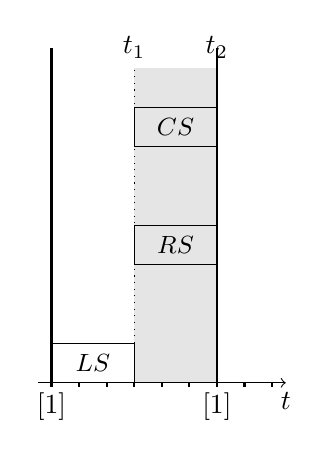
\begin{tikzpicture}[xscale=0.35,yscale=0.5]
   \node (O) at (0,0) {};
   \fill[gray!20!] (3.5,8) node[black,above] {$t_1$} node{} +(0,-8) 
   rectangle (6.5,8)  node[above,black] {$t_2$};
   \draw[dotted] (6.5,0) -- (6.5,8);
   \draw[dotted] (3.5,0) -- (3.5,8);
   \draw[->] (0,0) -- (9,0)  node[below] {$t$};
   \draw[thick] (6.5,0) node[below] {$\LE[1]$} -- (6.5, 8.5);
   \draw[thick] (0.5,0) node[below] {$\ES[1]$} -- (0.5, 8.5);
   \draw (0.5,0) rectangle (3.5,1) node[midway] {\small $LS$};
   \draw (3.5,3) rectangle (6.5,4) node[midway] {\small $RS$};
   \draw (3.5,6) rectangle (6.5,7) node[midway] {\small $CS$}; 

\foreach \i in {0.5,...,8.5} {
 \draw[thick] (\i,-0.1) -- (\i,0);
}
\end{tikzpicture}}
\hfill
  \subcaptionbox{activité $2$}[0.2\linewidth]{
  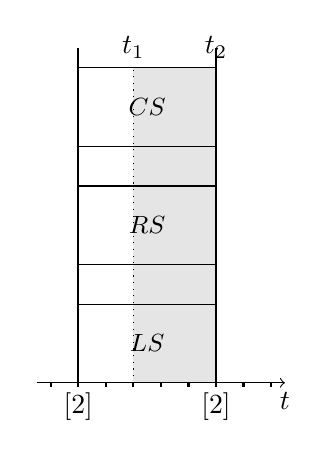
\begin{tikzpicture}[xscale=0.35,yscale=0.5]
    \node (O) at (0,0) {};
    \fill[gray!20!] (3.5,8) node[black,above] {$t_1$} node{} +(0,-8) 
    rectangle (6.5,8)  node[above,black] {$t_2$};
    \draw[dotted] (6.5,0) -- (6.5,8);
    \draw[dotted] (3.5,0) -- (3.5,8);
    \draw[->] (0,0) -- (9,0)  node[below] {$t$};
    \draw[thick] (6.5,0) node[below] {$\LE[2]$} -- (6.5, 8.5);
    \draw[thick] (1.5,0) node[below] {$\ES[2]$} -- (1.5, 8.5);
    \draw (1.5,0) rectangle (6.5,2) node[midway] {\small $LS$};
    \draw (1.5,3) rectangle (6.5,5) node[midway] {\small $RS$};
    \draw (1.5,6) rectangle (6.5,8) node[midway] {\small $CS$}; 

    \foreach \i in {0.5,...,8.5} {
      \draw[thick] (\i,-0.1) -- (\i,0);
    } 
  \end{tikzpicture}}
\hfill
\subcaptionbox{activité $3$}[0.2\linewidth]{
  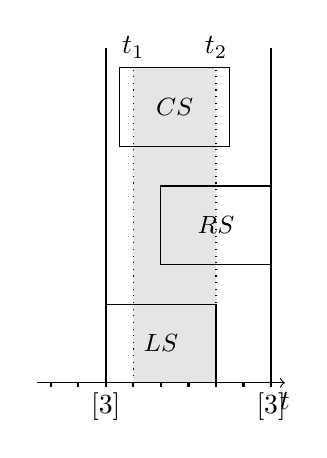
\begin{tikzpicture}[xscale=0.35,yscale=0.5]
    \node (O) at (0,0) {};
    \fill[gray!20!] (3.5,8) node[black,above] {$t_1$} node{} +(0,-8) 
    rectangle (6.5,8)  node[above,black] {$t_2$};
    \draw[dotted] (6.5,0) -- (6.5,8);
    \draw[dotted] (3.5,0) -- (3.5,8);
    \draw[->](0,0) -- (9,0) node[below] {$t$};
    \draw[thick] (8.5,0) node[below] {$\LE[3]$} -- (8.5, 8.5);
    \draw[thick] (2.5,0) node[below] {$\ES[3]$} -- (2.5, 8.5);
    \draw (2.5,0) rectangle (6.5,2) node[midway] {\small $LS$};
    \draw (4.5,3) rectangle (8.5,5) node[midway] {\small $RS$};
    \draw (3,6) rectangle (7,8) node[midway] {\small $CS$}; 

    \foreach \i in {0.5,...,8.5} {
      \draw[thick] (\i,-0.1) -- (\i,0);
    } 
  \end{tikzpicture}}
\hfill
\subcaptionbox{activité $4$}[0.2\linewidth]{
  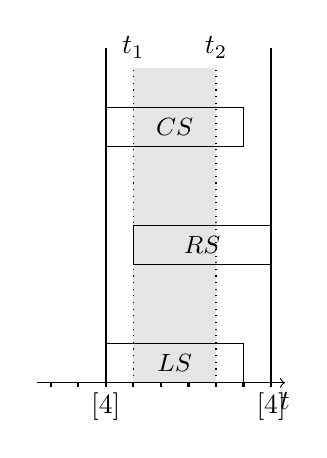
\begin{tikzpicture}[xscale=0.35,yscale=0.5]
    \node (O) at (0,0) {};
    \fill[gray!20!] (3.5,8) node[black,above] {$t_1$} node{} +(0,-8) 
    rectangle (6.5,8)  node[above,black] {$t_2$};
    \draw[dotted] (6.5,0) -- (6.5,8);
    \draw[dotted] (3.5,0) -- (3.5,8);
    \draw[->](0,0) -- (9,0)  node[below] {$t$};
    \draw[thick] (8.5,0) node[below] {$\LE[4]$} -- (8.5, 8.5);
    \draw[thick] (2.5,0) node[below] {$\ES[4]$} -- (2.5, 8.5);
    \draw (2.5,0) rectangle (7.5,1) node[midway] {\small $LS$};
    \draw (3.5,3) rectangle (8.5,4) node[midway] {\small $RS$};
    \draw (2.5,6) rectangle (7.5,7) node[midway] {\small $CS$};
    \foreach \i in {0.5,...,8.5} {
      \draw[thick] (\i,-0.1) -- (\i,0);
    } 
  \end{tikzpicture}}
\caption{Calcul de l'énergie minimale dans un intervalle $[t_1,t_2[$
  pour le \CUSP.}
\label{fig:ex_ER_CUSP}
\end{figure}

Le tableau suivant présente le calcul de l'énergie minimale de chaque
activité. Ces valeurs sont calculées à partir des
équations~\eqref{eq:LS_CUSP},~\eqref{eq:RS_CUSP}
et~\eqref{eq:CS_CUSP}.

\begin{center}
  \begin{tabular}{|P{1cm}|P{4cm}P{4cm}P{3.5cm}P{1.5cm}|}
    \hline
    act & \bbLS[i][3][6] & \bbRS[i][3][6] & \bbCS[i][3][6] & \bb[i][3][6]\\
    \hline
    1 & 1*(3-(3-0))=0 & 1*(3-(6-3))=3 & 1*(6-3)=3 & 0 \\
    2 & 2*(5-(3-1))=6 & 2*(5-(6-6))=10 & 2*(6-3)=6 & 6 \\    
    3 & 2*(4-(3-2))=6 & 2*(4-(8-6))=4 & 2*(6-3)=6 & 4 \\    
    4 & 1*(5-(3-2))=3 & 1*(4-(8-6))=3 & 1*(6-3)=3 & 3 \\    
    \hline
  \end{tabular}
\end{center}
La valeur de la fonction de marge $SL(3,6)$ est donc: 
\[\Big( 4*(6-3) \Big) - \Big( 0+6+4+3\Big) = 12 - 13 = -1 <0  \] 

L'instance n'est donc pas réalisable et une incohérence est détectée. 
\end{ex}

La règle de détection d'incohérence décrite par le
Théorème~\ref{th:centerRE} impose le calcul de la fonction de marge
pour tout intervalle $[t_1,t_2[ \in \mathbb{N}^2$, ce qui, en
pratique, n'est pas envisageable. Cependant, Baptiste {\it et al.} ont
proposé une caractérisation des intervalles sur lesquels il est
suffisant d'appliquer le raisonnement énergétique. Par suffisant, nous
entendons que, si une incohérence n'est pas détectée sur cet ensemble
d'intervalles, alors aucun autre intervalle ne permettra de conclure à
l'insatisfiabilité de l'instance. La taille de cet ensemble
d'intervalles d'{\it intérêt} est de l'ordre de $O(n^2)$. Le calcul de
la fonction de marge pouvant s'effectuer incrémentalement, la
complexité du checker énergétique est donc de $O(n^2)$.

Récemment, Derrien {\it et al.}~\cite{DP} ont proposé une
caractérisation plus fine de l'ensemble des intervalles d'intérêt pour
le raisonnement énergétique. L'ordre de grandeur de la taille de cet
ensemble d'intervalles n'est pas modifié et est toujours de l'ordre de
$n^2$ mais le nombre d'intervalles considérés est divisé par $7$. En
effet, la caractérisation de Baptiste {\it et al.} considère, pour
chaque paire d'activités, $15$ intervalles tandis que la
caractérisation de Derrien {\it et al.} n'en considère que $2$.


Ces caractérisations se basent toutes les deux sur l'idée suivante:
pour décider de l'existence d'un point $(t_1,t_2)$ pour lequel la
fonction de marge évaluée en ce point $SL(t_1,t_2)$ est négative, il
suffit d'évaluer la fonction en ses minima locaux. La principale
différence entre ces deux caractérisations est la caractérisation plus
ou moins fine de ces minima.

Nous allons brièvement détailler la caractérisation de Derrien {\it et
al.} que nous adapterons dans le cadre du \CECSP~dans le
chapitre~\ref{sec:PPC_CECSP}.

Pour étudier les minima locaux de la fonction de marge, les auteurs
de~\cite{DP} étudient les variations de cette dernière. L'expression
de la fonction de marge dépendant de $R(t_2-t_1)$ et de $\sum_{i \in
  \A} \bb$, ses variations dépendent des variations de la fonction
$(t_1,t_2) \rightarrow \sum_{i \in \A} \bb$. En particulier, ils
remarquent que tous les changements de variation de cette fonction ne
peuvent impliquer un minimum local. Pour qu'une variation implique un
tel minimum il faut que la dérivée à gauche de cette fonction soit
négative, que la dérivée à droite soit positive et qu'au moins l'une
d'entre elles soit non nulle. En effet, dans l'expression de la
fonction de marge, cette fonction est multipliée par $-1$.

Cette propriété, induite par le {\it test de la dérivée seconde}, leur
permet de décrire des conditions sur les consommations individuelles
des activités, $\bb$, sous lesquelles le point $(t_1,t_2)$ peut être
un minimum local de la fonction de marge. Ces conditions sont
exprimées dans le lemme~\ref{lem:min_CUSP}.

\begin{lemma}
\label{lem:min_CUSP}
Si le point $(t_1,t_2)$ est un minimum local de la fonction de marge
$SL(t_1,t_2)$, alors il existe deux activités $i$ et $j$ telles que les
conditions ci-dessous sont satisfaites. 
\begin{align} \frac{\delta^{-}\bb}{\delta t_1} &>
\frac{\delta^{+}\bb}{\delta t_1} \label{eq:deriv1_CUSP}\\ 
\frac{\delta^{-}\bb[j]}{\delta t_2}
& > \frac{\delta^{+}\bb[j]}{\delta t_2} \label{eq:deriv2_CUSP}
\end{align}
\end{lemma}

\begin{proof}
Soit $(t_1,t_2) \in \mathbb{N}^2$ tel qu'il n'existe aucune activité
$i$ vérifiant la condition~\eqref{eq:deriv1_CUSP}. Alors, $\sum_{i \in
  \A} \bb$ a sa dérivée à gauche supérieure à sa dérivée à droite. Par
le test de la dérivée seconde, un minimum local d'une fonction ne peut
exister que si la dérivée à gauche est plus grande que la dérivée à
droite. Donc le point $(t_1,t_2)$ ne peut pas être un minimum local. 

De la même façon, on peut prouver que si la
condition~\eqref{eq:deriv2_CUSP} n'est pas vérifiée, alors $(t_1,t_2)$
ne peut pas être un minimum local. 
\end{proof}

Le lemme~\ref{lem:min_CUSP} peut ensuite être utilisé pour établir 
les conditions nécessaires permettant de déterminer un l'ensemble des
intervalles d'intérêt. Pour cela, une étude des fonctions $t_1
\rightarrow \bb$ et $t_2 \rightarrow \bb$ est nécessaire. Nous montrons
comment obtenir une caractérisation des différentes dates de début
possibles pour un intervalle, la caractérisation des dates de fin
pouvant s'obtenir de manière similaire.

\begin{lemma}
  Pour chaque activité $i$ et pour tout début d'intervalle $t_1$ il
  existe au plus un intervalle $[t_1,t_2[$ tel que
  $\frac{\delta^{-}\bb}{\delta t_2} >
  \frac{\delta^{+}\bb}{\delta t_2} $:
  \begin{enumerate}
  \item si $t_1 \le \ES$ alors seulement l'intervalle $[t_1,\LE {[}$ doit
    être considéré.
  \item si $t_1  > \LS \land t_1 \ge \EE$ alors aucun intervalle ne
    doit être considéré. 
  \item si $t_1  > \LS \land t_1 <\EE \land t_1 < \LS$ alors seulement
    l'intervalle $[t_1,\ES+\LE-t_1 [$ doit
    être considéré.
  \item si $t_1  > \LS \land t_1 <\EE \land t_1 \ge \LS$ alors
    seulement l'intervalle $[t_1,\EE {[}$ doit
    être considéré.
  \end{enumerate}
\end{lemma}

\begin{proof}
Pour prouver ce lemme, nous étudions les variations de la fonction
$t_2 \rightarrow \bb$, à $t_1$ fixé. Les variations de cette fonction
dépendent de la position relative de $t_1$ par rapport à $\ES,\ \LS$ et
$\EE$. Le cas où $t_1 \le \ES$ est étudié ci-dessous et illustré pour une
activité $i$ possédant les caractéristiques suivantes: $\ES=2,\
\LE=8,\ p_i=4$ et $b_i=1$.

\begin{minipage}{\linewidth}
  \begin{minipage}{0.4\linewidth}
    \begin{itemize}
      
      \vspace{0.4cm}
    \item si $t_2 \le \LS$ alors $\bb=0$
      
      \vspace{0.4cm}
    \item si $\LS < t_2 < \LE$ alors $\bb= b_i (t_2 - \LS)$
      
      \vspace{0.4cm}
    \item si $\LE \le t_2 $ alors $\bb = p_i$
    \end{itemize}
  \end{minipage}
  \hfill
  \begin{minipage}{0.55\linewidth}
    \begin{figure}[H]
      \centering
      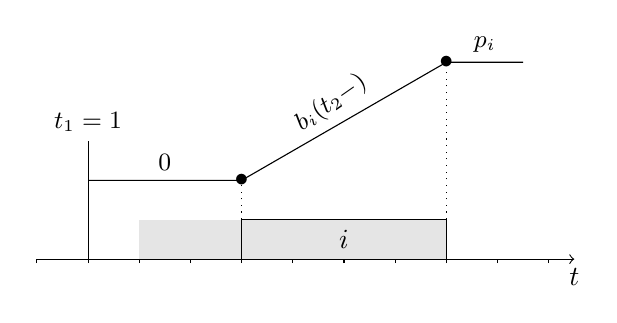
\begin{tikzpicture}      
        [yscale=0.5,xscale=0.65,
        every node/.style={color=black},%
        dot/.style={circle,fill=black,minimum size=4pt,inner sep=0pt,%
        outer sep=-1pt},
      cross/.style={path picture={ 
          \draw
          (path picture bounding box.south east) -- (path picture bounding box.north west) (path picture bounding box.south west) -- (path picture bounding box.north east);
        }}]
      \fill[gray!20] (2,0) rectangle (8,1);

      \node (O) at (0,0) {};
      \draw[->] (0,0) -- (10.5,0) node[below] {$t$}; 
\foreach \i in {0,1,...,10}{ \draw
        (\i,-0.1) -- (\i,0); }

      \draw (1,0) -- (1,3) node[above] {\small $t_1=1$}; 
      \draw (1,2) -- node[midway,above] {\small $0$} (4,2) node {$\bullet$} node[above] {\small $
        \LS$} -- node[midway,above,rotate=35] {\small $b_i(t_2 - \LS)$} (8,5)
      node {$\bullet$}  node[above] {\small $ \LE$} --
      node[midway,above] {\small $p_i$} (9.5,5) ;
      \draw[dotted] (4,0) -- (4,2);
      \draw[dotted] (8,0) -- (8,5);
      \draw (4,0) rectangle (8,1) node[midway] {$i$};
    \end{tikzpicture}
    \caption{{\'E}volution de la fonction de consommation minimale en
      fonction de $t_2$ pour le \CUSP.}
  \end{figure}
\end{minipage}
\end{minipage}

Le seul point $t_2$ pour lequel $ \frac{\delta^{-}\bb}{\delta t_2} >
\frac{\delta^{+}\bb}{\delta t_2}$ est $[1,8[= [t_1, \LE{[}$. 

Les trois autres cas peuvent être prouvés de façon très similaire. 
\end{proof}

Un raisonnement symétrique permet de caractériser l'ensemble des
points $t_1$ vérifiant la condition~\eqref{eq:deriv1_CUSP}. Une fois
que ces dates potentielles de début et de fin d'intervalle d'intérêt
sont caractérisées, elles sont rassemblées pour créer l'ensemble des
intervalles d'intérêt pour le raisonnement énergétique. 
La caractérisation complète de ces intervalles est décrite dans le
lemme suivant.

\begin{lemma}
  Si le point $(t_1,t_2)$ est un minimum local de la fonction de marge
$SL(t_1,t_2)$, alors il existe deux activités $i$ et $j$ telles que
$(t_1,t_2) \in \O_C(i,j)$ avec:
  
  \[ \O_C(i,j)= \left\{ 
      \begin{aligned} 
        &{[}\ES,\LE[j]{[} & \quad \text{ si }  \quad & \ES \le \ES[j] \ \land \
                                       \LE[j] \ge \LE \\
        &[\ES,\ES[j]+\LE[j]-\ES{[} & \quad \text{ si }  \quad &  \ES > \ES[j] \ \land \
                                                  \ES > \EE[j] \ \land \
                                                  \\
                                                 & & &\ES[j] + \LE[j] - \ES \ge \LE\\
        &[\ES,\EE[j]{[} & \quad \text{ si }  \quad &  \ES > \ES[j] \ \land \ \ES <
                                       \EE[j] \ \land \  \ES \ge \LS[j]
                                       \ \land \  \\
                                       & & &\EE[j] \ge \LE \\
        &[\LS,\LE[j]{[} & \quad \text{ si }  \quad &  \LS \le \ES[j] \ \land \
                                       \LE[j] < \LE \ \land \ \LE[j] >
                                       \LS \ \land \  \\
                                       &  & &\LE[j] \le \EE[j]\\
        &[\LS,\ES[j]+\LE[j]-\LS{[} & \quad \text{ si }  \quad &  \LS > \ES[j] \ \land \
                                                  \LE < \EE[j]\ \land \ \LS <
                                                  \LS[j] \ \land \ \\
                                              & & &\LS < \ES[j] +
\LE[j] - \LS \ \land \ \ES[j] + \LE[j] -\LS[i] < \LE\\
        &[\LS,\EE[j]{[} & \quad \text{ si }  \quad &  \LS > \ES[j] \ \land \
                                       \LS < \EE[j] \ \land \ \LS \ge
                                       \LS[j] \ \land \  \\
& & &\EE[j] < \LE\
                                       \land \ \EE[j] > \LS\ \land \ \EE[j] \le \EE\\
        &[\ES+\LE - \LE[j],\LE[j]{[} & \quad \text{ si }  \quad &  \LE[j] < \LE \
                                                    \land \  \LE[j] >
                                                    \LS \ \land \
                                                    \LE[j] > \EE \
                                                    \land \ \\
& & &
                                                    \ES+\LE-\LE[j] \le
                                                    \LS[j] \\
        &[\ES+\LE - \EE[j],\EE[j]{[} & \quad \text{ si }  \quad &  \EE[j] <\LE \
                                                    \land \ \EE[j] >
                                                    \LS \ \land \
                                                    \EE[j] > \EE \
                                                    \land \  \\
& & &\LS[j]
                                                    \le \ES +\LE -
                                                    \EE[j] < \EE[j] \
                                                    \land \ \\
& & &\LS[j] <
                                                    \ES+\LE - \EE[j]
      \end{aligned} 
    \right.
  \]
\end{lemma}

Une démonstration de ce lemme ainsi que la preuve que ces intervalles
sont suffisants pour détecter toute incohérence due au raisonnement
énergétique peut être trouvée dans~\cite{Alb}.

Grâce à cette caractérisation, l'algorithme de détection d'incohérence
de Baptiste {\it et al.} peut être amélioré. Pour cela, nous
considérons l'ensemble $\O_1=\cup_{i \in \A} \{\ES,\LS\}$ des dates de
début possibles d'un intervalle et l'ensemble $\O_2=\cup_{i \in \A}
\{\EE,\LE \}$ correspondant aux dates de fin. Ceci nous permet de
décrire l'algorithme (cf.~\ref{algo:check_CUSP}) de détection
d'incohérence en $O(n^2)$ de Derrien~\cite{Alb}.
\begin{algorithm}[!htb]
\setstretch{1.35}
  \caption{Algorithme de détection d'incohérence énergétique pour le \CUSP.}
  \label{algo:check_CUSP}
  \PourTous {$(i,t_1) \in \O_1$}{

    $pente=\sum_j \bb[j][t_1][t_1+1]$

    $SL_{ER}=0$, $t_2^{old}=t_1$

  \PourTous {$(j,t_2) \in \O_2 \cup \O_{t_1}$ par ordre croissant}{

    $SL_{ER}=SL_{ER}+pente*(t_2-t_2^{old})$

    \Si {$SL_{ER } > R(t_2-t_1)$}{
      Le problème est incohérent.}

    $pente=pente + \bb[j][t_1][t_2-1] - 2\bb[j] +  \bb[j][t_1][t_2+1]$

    $t_2^{old}=t_2$
  }
}
\end{algorithm}

Cette caractérisation peut aussi être étendue pour déterminer les
intervalles $(t_1,t_2)$ sur lesquels appliquer les ajustements du
raisonnement énergétique. Ces ajustements sont décrits par les 
règles~\ref{reg:ajust1_ER_CUSP} et~\ref{reg:ajust2_ER_CUSP}.  Dans la
règle~\ref{reg:ajust1_ER_CUSP}, nous imposons à une activité $i$ de
commencer après $t_1$ et si la quantité de ressource
disponible n'est pas suffisante pour ordonnancer les consommations
minimales de toutes les activités -- excepté celle de l'activité $i$
qui est remplacée par $\bbRS$ -- alors, nous pouvons déduire que
l'activité doit commencer avant $t_1$.

\begin{reg}
  \label{reg:ajust1_ER_CUSP}
  S'il existe un intervalle $[t_1,t_2[$ avec $t_1 > \ES$ et une activité $i$ pour lesquels:
  \[ \sum_{\substack{j \in \A \\ j \neq i}} \bb[j] + \bbRS > R (t_2-t_1)\]
  alors 
  \[  \LS \le t_1 - \frac{1}{b_i} \left( \sum_{\substack{j \in \A \\ j
          \neq i}} \bb[j] + \bbRS - R (t_2-t_1) \right) \]
\end{reg}

\begin{ex}
Considérons une ressource de capacité $R=3$ et les $4$ activités
suivantes: 
\begin{center}
  \begin{tabular}{|P{1cm}|P{1cm}P{1cm}P{1cm}P{1cm}|}
    \hline
    act & \ES & \LE & p_i & b_i  \\
    \hline
    1 & 0 & 6 & 5 & 2 \\
    2 & 2 & 6 & 1 & 3 \\    
    3 & 2 & 5 & 3 & 1 \\    
    4 & 0 & 4 & 2 & 1 \\    
    \hline
  \end{tabular}
\end{center}

Pour pouvoir ajuster la date de début au plus tard de l'activité $4$,
nous allons appliquer la règle~\ref{reg:ajust1_ER_CUSP} sur
l'intervalle $[2,4[$. Pour cela, nous commençons par calculer
la quantité de ressource requise par les activités dans cet intervalle. 

Pour l'activité $1$, cette quantité est $\bb[1][2][4]=4$. Elle est atteinte en
calant l'activité à gauche ou à droite (l'énergie est la même dans les
deux cas). Pour l'activité $2$, en calant l'activité à droite, nous
obtenons $\bb[2][2][4]=0$. Enfin, pour l'activité $3$, la quantité de
ressource requise vaut $\bb[3][2][4]=2$.

La quantité de ressource obtenue en calant l'activité $4$ à droite est de
$\bbRS[4][2][4]=2$. Nous devons ensuite comparer la somme de toutes
ces consommations, i.e. $4+0+2+2=8$, à la quantité de ressource
disponible dans l'intervalle $[2,4[$,
i.e. $R(t_2-t_1)=3*(4-2)=6$. Comme nous avons $6<8$, nous pouvons
appliquer la règle~\ref{reg:ajust1_ER_CUSP} et nous obtenons $\LS[4]
\le 2- (6 + 2 -6)  / 1 = 0$. Le domaine de la date de début de l'activité
$4$ est donc réduit à $\{0\}$.


\begin{figure}[!ht]
  \centering
  \subcaptionbox{l'activité $4$ ne peut commencer après $t_1=2$}[0.45\linewidth]{
    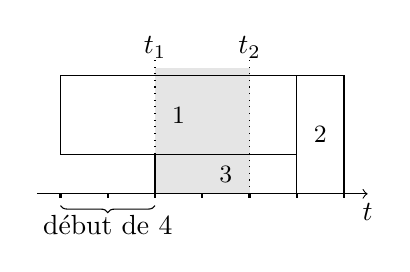
\begin{tikzpicture}[xscale=0.6,yscale=0.5  ,     every node/.style={color=black},%
      dot/.style={circle,fill=black,minimum size=4pt,inner sep=0pt,%
        outer sep=-1pt}, cross/.style={path picture={ \draw (path picture
          bounding box.south east) -- (path picture bounding box.north west)
          (path picture bounding box.south west) -- (path picture bounding
          box.north east); }}]
      \node (O) at (0,0) {};
      \fill[gray!20!] (2.5,3.2) node[black,above] {$t_1$} node{} +(0,-3.2) 
      rectangle (4.5,3.2)  node[above,black] {$t_2$};
      \draw[dotted] (4.5,0) -- (4.5,3.5);
      \draw[dotted] (2.5,0) -- (2.5,3.5);
      \draw[->] (0,0) -- (7,0) node[below] {$t$};
      \draw[decorate,decoration={brace,mirror}] (0.5,-0.3) --
      (2.5,-0.3) node[midway,below] {début de $4$};
      \draw (0.5,1) rectangle (5.5,3) node[midway] {\small $1$};
      \draw (5.5,0) rectangle (6.5,3) node[midway] {\small $2$};
      \draw (2.5,0) rectangle (5.5,1) node[midway] {\small $3$}; 
      
      \foreach \i in {0.5,...,6.5} {
        \draw[thick] (\i,-0.1) -- (\i,0);
      }
    \end{tikzpicture}}
  \hfill
  \subcaptionbox{le domaine de l'activité $4$ peut être ajusté}[0.45\linewidth]{
    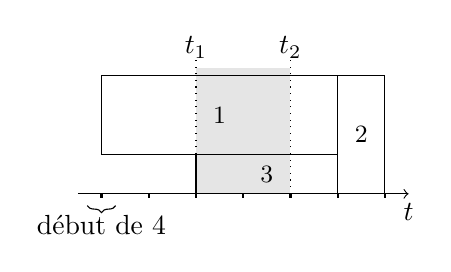
\begin{tikzpicture}[xscale=0.6,yscale=0.5  ,     every node/.style={color=black},%
      dot/.style={circle,fill=black,minimum size=4pt,inner sep=0pt,%
        outer sep=-1pt}, cross/.style={path picture={ \draw (path picture
          bounding box.south east) -- (path picture bounding box.north west)
          (path picture bounding box.south west) -- (path picture bounding
          box.north east); }}]
      \node (O) at (0,0) {};
      \fill[gray!20!] (2.5,3.2) node[black,above] {$t_1$} node{} +(0,-3.2) 
      rectangle (4.5,3.2)  node[above,black] {$t_2$};
      \draw[dotted] (4.5,0) -- (4.5,3.5);
      \draw[dotted] (2.5,0) -- (2.5,3.5);
      \draw[->] (0,0) -- (7,0)  node[below] {$t$};

      \draw[decorate,decoration={brace,mirror}] (0.2,-0.3) --
      (0.8,-0.3) node[midway,below] {début de $4$};
      \draw (0.5,1) rectangle (5.5,3) node[midway] {\small $1$};
      \draw (5.5,0) rectangle (6.5,3) node[midway] {\small $2$};
      \draw (2.5,0) rectangle (5.5,1) node[midway] {\small $3$}; 
      
      \foreach \i in {0.5,...,6.5} {
        \draw[thick] (\i,-0.1) -- (\i,0);
      }
    \end{tikzpicture}}
  \caption{Ajustement de borne du raisonnement énergétique pour le \CUSP.}
  \label{fig:ex_ER_CUSP}
\end{figure}

\end{ex}

Le même raisonnement que pour l'algorithme de détection d'incohérence
nous permet de caractériser l'ensemble des intervalles permettant de
réaliser des ajustements. Les conditions sous lesquelles un
intervalle peut conduire à un ajustement sont décrites dans le
lemme~\ref{lem:min_ajust_ER_CUSP}. Comment obtenir cette
caractérisation à partir de ce lemme sera aussi adapté dans le cadre
du \CECSP. De ce fait, elle n'est pas décrite ici.

\begin{lemma}
\label{lem:min_ajust_ER_CUSP}
  Si le point $(t_1,t_2)$ est un minimum local de la fonction
  $R(t_2-t_1) -\sum_{\substack{j \in \A \\ j \neq i}} \bb[j] - \bbRS
  $, alors une des conditions ci-dessous est satisfaite.
  \begin{align} 
    \exists (j,k), \ &~\frac{\delta^{-}\bb[j]}{\delta t_1}
    &>~&~\frac{\delta^{+}\bb[j]}{\delta t_1}
    &\land~&~\frac{\delta^{-}\bb[k]}{\delta t_2} & >~&
                                                       ~\frac{\delta^{+}\bb[k]}{\delta t_2} \label{eq:deriv1_adj_CUSP}\\
    \exists j , \ &~\frac{\delta^{-}\bb[j]}{\delta t_1}
    &>~&~\frac{\delta^{+}\bb[j]}{\delta t_1}
    &\land~&\frac{\delta^{-}\bbRS}{\delta t_2} & >~&
                                                        \frac{\delta^{+}\bbRS}{\delta t_2} \label{eq:deriv2_adj_CUSP}\\
    \exists k, \ &\frac{\delta^{-}\bbRS}{\delta t_1}
    &>~&\frac{\delta^{+}\bbRS}{\delta t_1}
    &\land~&~\frac{\delta^{-}\bb[k]}{\delta t_2} & >~&
                                                       ~\frac{\delta^{+}\bb[k]}{\delta t_2} \label{eq:deriv3_adj_CUSP}\\
                     &\frac{\delta^{-}\bbRS}{\delta t_1}
    &>~&\frac{\delta^{+}\bbRS}{\delta t_1}
    &\land~&\frac{\delta^{-}\bbRS}{\delta t_2} & >~&
                                                        \frac{\delta^{+}\bbRS}{\delta t_2} \label{eq:deriv4_adj_CUSP}
  \end{align}
\end{lemma}

L'ordre de grandeur de l'ensemble des intervalles d'intérêt pour les
ajustements est aussi de $n^2$ et l'algorithme permettant de procéder
à tous les ajustements possibles a une complexité en $O(n^3)$. Ceci
fait du raisonnement énergétique un des moins algorithmes de filtrage
utilisés en pratique, même si ce raisonnement est un des plus forts
pour la contrainte cumulative.


De manière similaire à la règle~\ref{reg:ajust1_ER_CUSP}, une autre
règle permettant d'ajuster la date de début au plus tôt d'une activité
peut être déduite.

\begin{reg}
  \label{reg:ajust2_ER_CUSP}
  S'il existe un intervalle $[t_1,t_2[$ avec $t_1 > \ES$ et une
activité $i$ pour lesquels:
  \[ \sum_{\substack{j \in \A \\ j \neq i}} \bb[j] +
    \min(\bbCS,\bbLS) > R (t_2-t_1)\] 
  alors 
  \[  \ES \ge t_2 - \frac{1}{b_i} \left(R (t_2-t_1)  -\sum_{\substack{j \in \A \\ j
          \neq i}} \bb[j]  \right) \]
\end{reg}

Le lemme~\ref{lem:min_ajust_ER_CUSP} peut aussi être appliqué dans ce
cas, en considérant la fonction suivante au lieu de $\bbRS$:
$b_i*\max\Big(\, 0\, , \, \min(\, \LE\, ,\, t_2\,) - \max(\, \LS\, ,
  \, t_1\,) \,\Big)$. 


Les différentes règles de filtrages présentées dans les paragraphes
précédents ont parfois été étendues ou couplées afin de définir de
nouvelles règles plus fortes que considérées indépendamment. Certaines
d'entre elles sont décrites dans le paragraphe suivant. 


\subsubsection{Règles de filtrage étendues}
\label{sec:mix_CUSP}

Parmi les règles de filtrage étendues ou couplées on trouve le
raisonnement Edge-Finding étendu~\cite{ExtEF}, le
Time-Table-Edge-Finding~\cite{V11} ou encore le Time-Table
disjonctif~\cite{Gay2015}. Dans ce paragraphe, nous montrerons comment
coupler deux raisonnements en présentant, en premier lieu, l'idée de
la méthode utilisée pour le Time-Table-Edge-Finding et, dans un second
temps, en détaillant celle utilisée pour le Time-Table disjonctif. En
effet, une adaptation sera présentée dans le
chapitre~\ref{sec:PPC_CECSP} dans le cadre du \CECSP.

L'idée du Time-Table-Edge-Finding est de renforcer le raisonnement
existant du Edge-Finding en prenant en considération le profil
obligatoire de la ressource. L'algorithme proposé par Vil{\'i}m est en
$O(n^2)$ et est un des plus performants en pratique pour résoudre les
problèmes cumulatifs. 

Afin d'ajouter l'énergie déduite du raisonnement Time-Table à celle du
raisonnement Edge-Finding, les activités sont séparées en deux
parties, la partie obligatoire et la partie libre. Ceci permet
d'éviter de comptabiliser l'énergie deux fois lors du calcul de cette
dernière. L'énergie consommée par un ensemble d'activités dans un
intervalle est alors égale à la somme des énergies des parties libres
de ces dernières et de la fonction de profil obligatoire de la
ressource à l'intérieur de cet intervalle. 

Dans le même esprit, Gay~\cite{Gay2015} propose de combiner le
raisonnement disjonctif et le raisonnement Time-Table. Pour ce faire,
l'auteur définit la notion d'{\it intervalle minimum de
superposition}. Cette notion va permettre de définir une nouvelle
règle de filtrage dans le cas où faire débuter une activité $j$ à sa
date de début au plus tôt $\ES[j]$ implique que cette activité
chevauchera forcément une activité $i$ vérifiant $b_i+b_j > R$ dans
tout ordonnancement réalisable. Ceci est dû au fait que la fenêtre de
temps de $j$ ne peut contenir un point que l'activité $i$ devra
forcément chevaucher. Quand l'activité $i$ n'a pas de partie
obligatoire, l'intervalle que $j$ ne peut intersecter peut être
caractérisé.

\begin{defi}
\label{des:moi_CUSP} 
L'intervalle minimal de superposition d’une activité $i$, noté
$moi_i$, est l’intervalle de temps le plus petit tel que $i$ s’exécute
au moins durant un point de temps de cet intervalle, et ce
indépendamment du moment auquel l'activité $i$ est exécutée.  

Formellement,  l’intervalle minimal de superposition est défini par
$[\EE-1,\LS{]}$.
\end{defi}

Quand une activité possède une partie obligatoire, elle ne possède pas
d'intervalle minimum de superposition. 

\begin{ex}
La figure~\ref{fig:moi_CUSP} illustre l'intervalle minimum de
superposition d'une activité $i$ ne possédant pas de partie
obligatoire. \begin{figure}[!htb]
  \begin{center}
    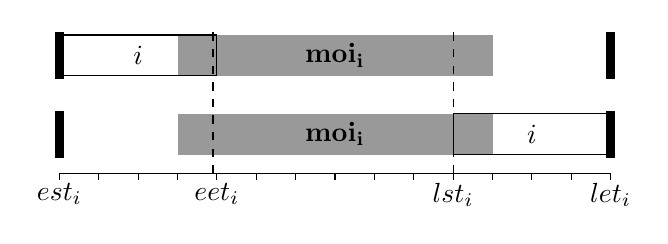
\begin{tikzpicture}
      [xscale=0.5, yscale= 0.4,node distance=0.5cm][decoration={brace}]
      \node (sil) at (0,0) {} ;
      \node (sir) at (10,0) {}; 
      \draw (10,0) node[below] {$lst_i$};
      \node (eir) at (14,0) {} ;
      \node (eil) at (4,0) {} ;
      \draw (4,0) node [below]  {$eet_i$} ;
    %  \node [below of=eil]  {$eet_i$}; 
    %  \node[below of= sir] {$lst_i$};
      \draw (sil.center) node[below] {$est_i$}--
      (eir.center) node[below] {$let_i$};
      
      \draw[line width=3pt] (0,0.5) -- (0,2);
      \draw[line width=3pt] (14,0.5) -- (14,2);
      \draw[line width=3pt] (0,3) -- (0,4.5);
      \draw[line width=3pt] (14,3) -- (14,4.5);

      \fill[gray!80] (3,0.6) rectangle (11,1.9) node[midway,color=black] {$\mathbf{moi_i}$};
      \fill[gray!80] (3,3.1) rectangle (11,4.4) node[midway,color=black] {$\mathbf{moi_i}$};
      
      \draw (0,3.1) rectangle (4,4.4) node[midway] {$i$};
      \draw (10,0.6) rectangle (14,1.9) node[midway] {$i$};

      \draw[dashed] (3.9,0) -- (3.9,4.5);
      \draw[dashed] (10,0) -- (10,4.5);

      \foreach \i in {0,...,14} {
        \draw (\i,0)  -- (\i,-0.2);
      }
    \end{tikzpicture}
  \end{center}

  \caption{Intervalle minimum de superposition d'une activité pour le \CUSP.}
  \label{fig:moi_CUSP}
\end{figure}
\end{ex}

Cette notion permet de définir une première règle d'ajustement. Cette
règle sera améliorée dans un second temps. 

\begin{reg}
\label{reg:RDR_CUSP}
  Soient deux activités $i$ et $j$ telles que $i$ ne possède pas de
  partie obligatoire et $b_i+b_j > R$. Si ordonnancer l'activité
 $j$ à sa date de début au plus tôt la fait se superposer complètement
 à l’intervalle minimal de superposition de $i$ ($moi_i \subseteq
 [\ES[j],\EE[j]{]}$), alors $\ES[j] \ge \EE$.
\end{reg}

\begin{ex}
La règle~\ref{reg:RDR_CUSP} est illustrée par la
figure~\ref{fig:RDR_CUSP}. Dans la partie gauche de la figure, on
peut constater que les activités $i$ et $j$ ne peuvent être exécutées
en parallèle à cause de la capacité de la ressource. Si l'activité $j$
commence à $\ES[j]$, alors elle intersecterait complètement $moi_i$ et
il serait impossible d'ordonnancer $i$. Sur la partie droite de la
figure, $\ES[j]$ a été ajusté et l'activité $j$ ne peut commencer
avant $\min\{t \in \H|t \in moi_i \}$.
  \begin{figure}[!htb]
    \centering
    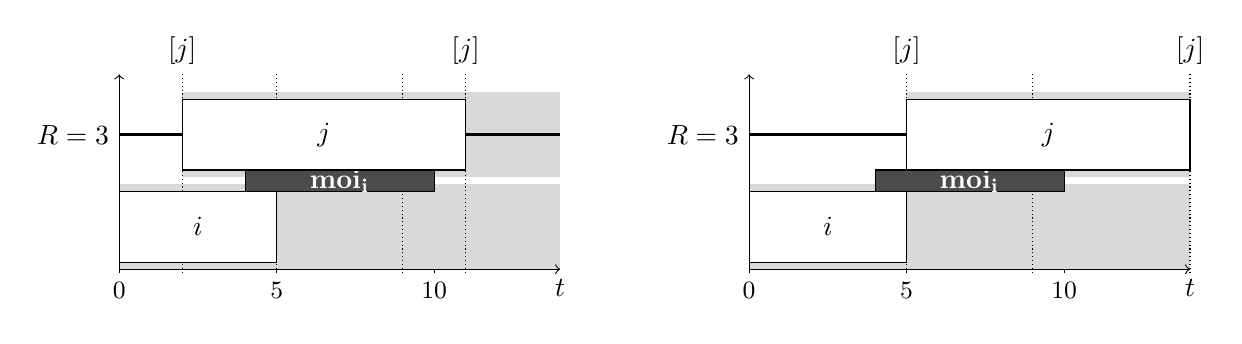
\begin{tikzpicture}
      \begin{scope} [yscale=0.45,xscale=0.4]
        \node (O) at (0,0) {};

        \foreach \i in {0,5,...,10} {
          \draw (\i,0) -- (\i,-0.1) node[below] {\small $\i$};
        }
        \fill[gray!30] (0,0) rectangle (14,2.4);
        \fill[gray!30] (2,2.6) rectangle (14,5);
        \draw[thick] (0,3.8)  node[left] {$R=3$} -- (14,3.8);
        
        
        \draw[densely dotted] (2,-0.1) -- (2,5.5) node[above] {$\ES[j]$};
        \draw[densely dotted] (11,-0.1) -- (11,5.5) node[above] {$\EE[j]$};
        \draw[densely dotted] (5,-0.1 ) node[below=0.3cm] {$\EE$}-- (5,5.5) ;
        \draw[densely dotted] (9,-0.1) node[below=0.3cm] {$\LS$} --
        (9,5.5) ;

        \draw[fill=black!70!] (4,2.2) rectangle
        (10,2.8) node[midway,white] {$\mathbf{moi_i}$};
        \draw[fill=white] (0,0.2) rectangle (5,2.2) node[midway]
        {$i$};

        \draw[fill=white] (2,2.8) rectangle (11,4.8) node[midway]
        {$j$};

        \draw[->] (0,0) -- (14,0) node[below] {$t$};
        \draw[->] (0,0) -- (0,5.5) ;
        % \draw[densely dotted] (6,-0.1) -- (6,5.5) node[above] {$\ES[j]^{'}$};
        % \draw[->] (1.8,5.8) -- (5.2,5.8);
      \end{scope}     
      \begin{scope} [yscale=0.45,xscale=0.4,xshift=20cm]
        \node (O) at (0,0) {};
        \foreach \i in {0,5,...,10} {
          \draw (\i,0) -- (\i,-0.1) node[below] {\small $\i$};
        }

        \fill[gray!30] (5,2.6) rectangle (14,5);
        \fill[gray!30] (0,0) rectangle (14,2.4);
        \draw[thick] (0,3.8)  node[left] {$R=3$} -- (14,3.8);
        
        \draw[densely dotted] (14,-0.1) -- (14,5.5) node[above] {$\EE[j]$};
        \draw[densely dotted] (5,-0.1 ) node[below=0.3cm] {$\EE$}-- (5,5.5) node[above] {$\ES[j]$};
        \draw[densely dotted] (9,-0.1) node[below=0.3cm] {$\LS$} -- (9,5.5) ;
        \draw[fill=black!70!] (4,2.2) rectangle
        (10,2.8) node[midway,white] {$\mathbf{moi_i}$};
        
        \draw[fill=white] (0,0.2) rectangle (5,2.2) node[midway]
        {$i$};
        \draw[fill=white] (5,2.8) rectangle (14,4.8) node[midway]
        {$j$};


        \draw[->] (0,0) -- (14,0)  node[below] {$t$};
        \draw[->] (0,0) -- (0,5.5) ;
        % \draw[densely dotted] (6,-0.1) -- (6,5.5) node[above] {$\ES[j]^{'}$};
        % \draw[->] (1.8,5.8) -- (5.2,5.8);  

      \end{scope}
    \end{tikzpicture}
    \caption{Illustration de la règle~\ref{reg:RDR_CUSP} pour le \CUSP.}
    \label{fig:RDR_CUSP}
  \end{figure}
\end{ex}

Nous montrons maintenant comment les auteurs de~\cite{Gay2015}
intègrent les informations déduites du Time-Table pour proposer une
règle de filtrage plus forte que celle décrite ci-dessus. Cette règle
sera décrite seulement dans le cas où les activités $i$ et $j$ ne
possèdent pas de partie obligatoire. Le cas inverse est décrit
dans~\cite{Gay2015} et repose sur la séparation des activités en une
partie obligatoire et une partie libre.


La règle~\ref{reg:RDR_CUSP} compare seulement les consommations de $i$
et de $j$ avec la capacité de la ressource $R$. Cependant, les
consommations obligatoires des autres activités peuvent ne pas laisser
$R$ unités de ressource durant l'intersection de $i$ et de $j$. La
règle suivante prend donc en considération le profil obligatoire de la
ressource.

\begin{reg}
\label{reg:TTDR_CUSP}
Soient $i$ et $j$ deux activités qui ne possèdent pas de partie
obligatoire et telles que $ b_i +b_j + \min_{t \in moi_i} TT_{\A}(t) >
R$.   Si ordonnancer l'activité
 $j$ à sa date de début au plus tôt la fait se superposer complètement
 à l’intervalle minimal de superposition de $i$ ($moi_i \subseteq
 [\ES[j],\EE[j]{]}$), alors $\ES[j] \ge \EE$.
\end{reg}

\begin{ex}
  Considérons les activités suivantes: 

  \vspace{-0.5cm}
  \begin{center}
    \begin{tabular}{|P{1cm}|P{1cm}P{1cm}P{1cm}P{1cm}|}
      \hline
      act &\ES & \LE & p_i & b_i  \\
      \hline
      1 & 2 & 11 & 3 & 2 \\
      2 & 1 & 20 & 9 & 1 \\
      3 & 2 & 11 & 9 & 1 \\
      \hline
    \end{tabular}
  \end{center}

  Les activités $1$ et $2$ ne possèdent pas de partie obligatoire tandis
  que l'activité $3$ est forcément en cours d'exécution durant
  l'intervalle $[2,11[$. 

  \begin{figure}[!htb]
    \centering
    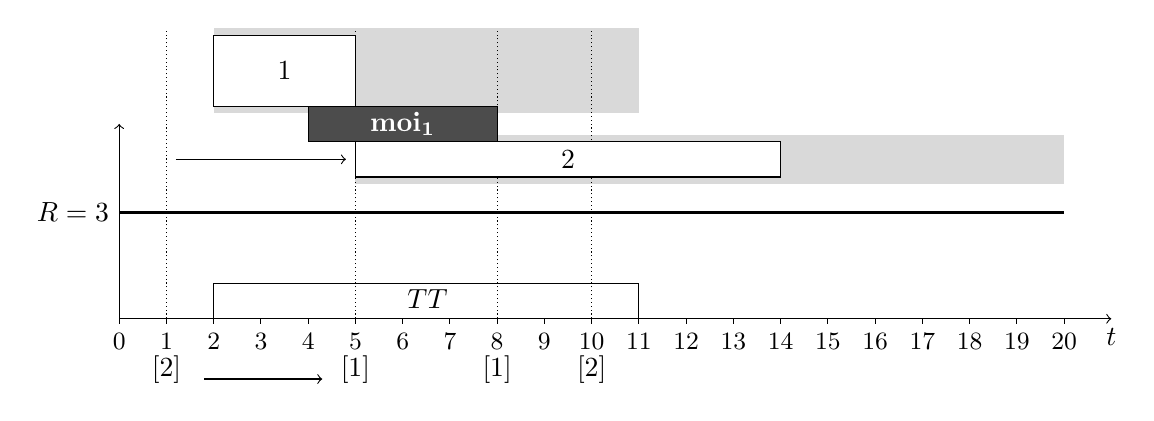
\begin{tikzpicture}
      [yscale=0.45,xscale=0.6]
      \node (O) at (0,0) {};
      \foreach \i in {0,1,...,20} {
        \draw (\i,0) -- (\i,-0.15) node[below] {\small $\i$};
      }
      
      \draw (2,0) rectangle (11,1) node[midway] {$TT_{\A}$};
      \fill[gray!30] (5,3.8) rectangle (20,5.2);
      \fill[gray!30] (2,5.8) rectangle (11,8.2);
      
      \draw [->] (1.2,4.5) -- (4.8,4.5);
      \draw [->] (1.8,-1.7) -- (4.3,-1.7);
      \draw[densely dotted] (1,-0.1) node[below=0.3cm] {$\ES[2]$}-- (1,8.2) ;
      \draw[densely dotted] (5,-0.1 ) node[below=0.3cm] {$\EE[1]$}--
      (5,8.2);
      \draw[densely dotted] (10,-0.1) node[below=0.3cm] {$\EE[2]$} -- (10,8.2) ;
      \draw[densely dotted] (8,-0.1) node[below=0.3cm] {$\LS[1]$} -- (8,8.2) ;
      
      \draw[fill=black!70!] (4,5) rectangle
      (8,6) node[midway,white] {$\mathbf{moi_1}$};
      
      \draw[fill=white] (2,6) rectangle (5,8) node[midway]
      {$1$};
      \draw[fill=white] (5,4) rectangle (14,5) node[midway]
      {$2$};
      
      \draw[->] (0,0) -- (21,0) node[below] {$t$};
      \draw[->] (0,0) -- (0,5.5) ;
       \draw[thick] (0,3)  node[left] {$R=3$} -- (20,3);
       % \draw[densely dotted] (6,-0.1) -- (6,5.5) node[above] {$\ES[j]^{'}$};
      % \draw[->] (1.8,5.8) -- (5.2,5.8);  
    \end{tikzpicture}
    \caption{Illustration du Time-Table disjonctif dans le cadre du \CUSP.}
    \label{fig:TTDR_CUSP}
  \end{figure}
L'intervalle $moi_1=[4,9[$ est complètement inclus dans l'intervalle
formé par $\ES[2]$ et $\EE[2]$, i.e. $[1,10[$. De plus, le minimum du
profil de consommation de la ressource dans $moi_1$ est de $1$. Donc,
les activités $1$ et $2$, consommant respectivement $2$ et $1$ unités
de ressource, ne peuvent se chevaucher sur l'intervalle $[4,9[$. Donc
$\ES[2]$ peut être ajusté à $5$. 
\end{ex}

On peut remarquer qu'aucun des autres raisonnements présentés dans ce
chapitre n'aurait filtré de valeurs du domaine de $st_2$. En
particulier, le raisonnement énergétique  ne détecte
pas d'ajustement dans ce cas. Le raisonnement Time-Table disjonctif
n'est donc dominé par aucun autre raisonnement existant. 




